\documentclass[bachelor, och, coursework ]{SCWorks}
% параметр ---тип обучения ---одно из значений:
%    spec     ---специальность
%    bachelor ---бакалавриат (по умолчанию)
%    master   ---магистратура
% параметр ---форма обучения ---одно из значений:
%    och   ---очное (по умолчанию)
%    zaoch ---заочное
% параметр ---тип работы ---одно из значений:
%    referat    ---реферат
%    coursework ---курсовая работа (по умолчанию)
%    diploma    ---дипломная работа
%    pract      ---отчет по практике
%    pract      ---отчет о научно-исследовательской работе
%    autoref    ---автореферат выпускной работы
%    assignment ---задание на выпускную квалификационную работу
%    review     ---отзыв руководителя
%    critique   ---рецензия на выпускную работу
% параметр ---включение шрифта
%    times    ---включение шрифта Times New Roman (если установлен)
%               по умолчанию выключен
\usepackage{amsmath}
\usepackage[T2A]{fontenc}
\usepackage[utf8]{inputenc}
\usepackage{graphicx}
\usepackage[sort,compress]{cite}
\usepackage{amsmath}
\usepackage{amssymb}
\usepackage{amsthm}
\usepackage{fancyvrb}
\usepackage{longtable}
\usepackage{array}
\usepackage{caption}
\usepackage[english,russian]{babel}
\captionsetup[figure]{font= normalsize, labelfont=normalsize}
\DeclareUnicodeCharacter{00A0}{ }

\usepackage[colorlinks=true]{hyperref}
\usepackage{float}
\usepackage{caption}
\captionsetup[figure]{font= normalsize, labelfont=normalsize}


\begin{document}

% Кафедра (в родительном падеже)
\chair{Дискретной математики и информационных технологий}

% Тема работы
\title{Разработка приложения для частотного анализа новостных сообщений}

% Курс
\course{3}

% Группа
\group{322}

% Факультет (в родительном падеже) (по умолчанию "факультета КНиИТ")
%\department{факультета КНиИТ}

% Специальность/направление код ---наименование
%\napravlenie{02.03.02 "-----Фундаментальная информатика и информационные технологии}
%\napravlenie{02.03.01 "-----Математическое обеспечение и администрирование информационных систем}
\napravlenie{09.03.01 "---Информатика и вычислительная техника}
%\napravlenie{09.03.04 "-----Программная инженерия}
%\napravlenie{10.05.01 "-----Компьютерная безопасность}

% Для студентки. Для работы студента следующая команда не нужна.
%\studenttitle{Студентки}

% Фамилия, имя, отчество в родительном падеже
\author{Конорова Дмитрия Аркадьевича}

% Заведующий кафедрой
\chtitle{доцент, к.\,ф.-м.\,н.} % степень, звание
\chname{Л.\,Б.\,Тяпаев}

%Научный руководитель (для реферата преподаватель проверяющий работу)
\satitle{доцент, к.\,э.\,н.} %должность, степень, звание
\saname{Г.\,Ю.\,Чернышова}


% Семестр (только для практики, для остальных
% типов работ не используется)
\term{}

% Наименование практики (только для практики, для остальных
% типов работ не используется)
%\practtype{}

% Продолжительность практики (количество недель) (только для практики,
% для остальных типов работ не используется)
\duration{}

% Даты начала и окончания практики (только для практики, для остальных
% типов работ не используется)
\practStart{}
\practFinish{}

% Год выполнения отчета
\date{2024}




\maketitle

% Включение нумерации рисунков, формул и таблиц по разделам
% (по умолчанию ---нумерация сквозная)
% (допускается оба вида нумерации)
%\secNumbering


\tableofcontents


% Раздел "Обозначения и сокращения". Может отсутствовать в работе


% Раздел "Определения". Может отсутствовать в работе
%\definitions

% Раздел "Определения, обозначения и сокращения". Может отсутствовать в работе.
% Если присутствует, то заменяет собой разделы "Обозначения и сокращения" и "Определения"
%\defabbr


% Раздел "Введение"
\intro
Для анализа инновационной деятельности региональных субъектов применяются традиционные подходы основанные на комплексной оценке статистических показателей инновационного развития .................. 




В век огромного количества информации очень важно уметь быстро и качественно её анализировать. В этом помогает подход частотного анализа, который основан на частоте встречаемости слов в корпусе текстов. 

Цель работы --- применение частотного анализа для оценки новостных документов. 
Объектом исследования являются методы машинного обучения для работы с текстовыми документами.
Предметом исследования является использование информационных технологий Text Mining для анилиза новостных сообщений. 
Задачи курсовой работы представлены следующим образом:
\begin{itemize}
    \item анализ подходов к формированию облака слов;
    \item разработка приложения для частотного анализа новостных документов;
    \item применение разработанного подхода для сравнительной оценки региональных новостных сообщений за различные периоды.
\end{itemize}




\section{Формирование облака слов для облака текстовых документов}
\subsection{Подходы к формированию облака слов}

Облако слов --- это инструмент для визуализации текстов. От веса или частоты встречаемости слова в тексте зависит его размер и цвет в визуализации. Чем больше слово используется в тексте, тем более крупным шрифтом оно будет отражено. Облако слов позволяет определять ключевые слова в тексте, а по ним можно определить тематику текста.
Одним из преимуществ облака слов является то, что с его помощью можно сравнивать тексты. 
Облако слов --- это эффективный инструмент для обучения студентов, школьников и не только. Оно помагает заинтересовать учащихся в изучении рассматриваемой темы.

Для формирования облака слов используются различные подходы. Рассмотрим некоторые из них.
Частотный анализ --- подход, который для каждого слова вычисляет то, сколько раз слово встречалось в тексте. На основе этих данных строится облако слов.
Семантический анализ --- подход, который учитывает не только частоту встречаемости слова в тексте, но и его значение и контект, в котором оно встречается.
Тематический анализ --- подход, который позволяет выделить в тексте основные темы и отображать только те слова, которые принадлежат вабранным пользователем темам.
Машинное обучение --- подход, который использует алгоритмы машинного обучения. Например, для выявления ключевых слов в тексте могут использоваться алгоритмы классификации и кластеризации.
Ручное составление слов, которые будут отображены в облаке, позволяет гибко убирать нежелаемые слова.

Конечный выбор подхода к формированию облака слов зависит от целей и задач, которые ставятся перед пользователем. Кроме того, важным фактором при выборе подхода является объем текста, который необходимо обработать. 

Формирование облака слов --- это эффективный способ визуализации информации, который может быть использован для анализа текста, выявления ключевых слов и тем, а также для презентации результатов исследования. При правильном выборе подхода и инструментов формирование облака слов может занять минимум времени и достичь максимальной эффективности.

Для формирования облака слов необходимо подговить исходный текст. Необходимо удалить знаки препинания, цифры и специальные символы, привести слова к нижнему регистру, провести токенизацию, то есть разделение текста на слова. Также нужно привесте к нормальной форме, то есть провести лемматизацию.
Для глагола нормальная форма --- инфинитив, для существительного --- именительный падеж и единственное число, для прилагательного --- именительный падеж, мужской род и единственной число. 
После приведения слов к нормальной форме необходимо удалить стоп-слова, которые не несут смысловой нагрузки. Это местоимения, союзы, предлоги и другое. Для каждого из оставшихся слов нужно посчитать, сколько раз оно встречается в получившемся списке слов. На основе данной частотной таблице строится облако слов.

В языках со сложным словообразованием, таких как русский, могут понадобиться дополнительные словари, которые учитывают особенности речи. К процессу лемматизации также могут быть подключены словари сленга, аббревиатур и сокращений, чтобы корректно обрабатывать такие типы слов.

Таким образом, этапы формирования облака слов выглядят следующим образом: 
\begin{enumerate}
    \item[1)] считывание текста;
    \item[2)] удаление знаков препинания, цифр и специальных символов;		
    \item[3)] приведение символов к нижнему регистру;
    \item[4)] токенизация;
    \item[5)] лемматизация;
    \item[6)] удаление стоп-слов;
    \item[7)] расчет частоты употребляемости слов в полученном тексте;
    \item[8)] создание облака слов.
\end{enumerate}

Далее в работе будут реализованы данные этапы формирования облак слов.







\subsection{Применение облака слов для анализа документов}
Рассмотрим несколько способов применения облака слов в исследовательской работе и процессе обучения\cite{1}:
\begin{itemize} 
    \item компрессия информации для первичного восприятия текста и его последующего воспроизведения; 
    \item анализ текста через определение частотности активных лексем, выделение ключевых слов;
    \item сопоставление текстов посредством облака слов;
    \item сопоставление облака с другими видами репрезентации сжатой информации; 
    \item визуальная репрезентация текста как альтернатива диаграмме;
    \item создание инфографики на основе информации, представленной в облаке; 
    \item организация и контроль обратной связи (ключевые слова урока, проекта, курса); 
    \item мозговой штурм; 
    \item моделирование или восстановление содержания текста по облаку слов;
    \item репрезентация отчета и результатов исследования;
    \item определение приоритетных направлений учебных программ или планов;
    \item составление словаря наиболее частотных терминов, функционирующих в научном тексте; 
    \item интерполяция текстовых фраз в форме облака в видео; 
    \item репрезентация научной информации, лекций, теоретического материала, правил в виде облака (ключевые слова будут выделены и более заметны, чем просто перечень правил).
\end{itemize}

Компрессия текста – это извлечение из текста основной информации, то есть информации, без которой нарушается логика изложения.


  Формирование облака слов обеспечит возможность на основе новостных сообщений, обзоров в социальных сетях определить трендовые темы, тенденции и проблемные области не только для отдельных отраслей, но и для регионов в целом. 

В \cite{2} используется облако слов как средство формирования лексических навыков учащихся на уроках английского языка. Выдержка из статьи: “Облако слов как средство обучения помогает разнообразить процесс обучения”, “Автор приходит к выводу, что облако слов представляет собой необычное и полезное средство обучения лексике, вызывающее интерес, как со стороны учителя, так и со стороны учащихся. Облако слов успешно применяется в изучении большинства тем и практически на всех этапах урока.” 

“На основе частотных таблиц строятся графические представления в виде “облака” слов, где размер шрифта отражает частоту использования этого слова в тексте. Такая картина даёт общее представление о ядре дискурса, о тех словах, которые употребляются чаще других”\cite{3}.  


 В \cite{4} представлено предварительное исследование о влиянии облаков слов на критическое мышление, когда они включаются в онлайн-дискуссии. В ходе онлайн-дискуссии студентам было предложено критически проанализировать две речи, которым было присвоено одно из двух условий: одно, в котором текст был линейным, и другое, в котором текст был представлен в виде облаков слов. Посты для обсуждения были закодированы в двух смешанных разделах курса антропологии для студентов, чтобы оценить тип и частоту демонстрируемого в них критического мышления. Учащиеся в режиме “облако слов” демонстрировали больше примеров критического мышления, чем учащиеся в линейном режиме, и чаще сочетали изложение мысли с цитированием доказательств. Статья завершается рекомендациями для других педагогов, заинтересованных во внедрении аналогичного подхода.

В \cite{5} применяется облако слов для привлечения внимания исследователей к исследованию шейной цервиальной миелопатии. Для этого был проведен онлайн-опрос, в котором было предложено людям с данным заболеванием предложить свои слова и проголосовать за слова, с которыми у них оссоциируется эта болезнь. После проверки уточненный список слов был повторно выставлен в виде оналйн-опроса для голосования. На основе результатов опросов были сгенерированы облака слов.

После первого опроса было представлено семьдесят девять терминов. Затем был повторный опрос, в котором было восемьдесят семь уточненных слов (в результате чего было добавлено еще 39 слов). Были сгенерированы четыре облака слов по категориям диагностика, лечение, долгосрочные последствия и другие. Для группы ``диагностика'' наболее частые слова по результатам опросов: слабость, боль, дисбаланс; для группы ``лечение'': хирургия, боль; для группы ``долгосрочные последствия'': инвалидность, усталость; для группы ``другое'': незнание. 

В \cite{6} исследуется отношение людей к компании по вакцинации от COVID-19 на основе постов социальной сети Twitter о вакцинах от COVID. Данные посты были разделены по отношению людей к вакцинации на 3 категории: положительные, нейтральные и отрицательные. Для каждой из этих категорий было сформировано облако слов с использованием масок для визуализации результата исследования.









Существуют такие методы векторизации:
{\begin{itemize}
    \item Bag of words;
    \item hot vectors;
    \item TF-IDF;
    \item word2vec;
    \item GLOVE;
    \item Fast text;
    \item CBOW.
\end{itemize}}


TF-IDF (term frequency - inverse document term frequency) --- это статистический показатель, применяемый для оценки важности слова в контексте категории, документа или коллекции документов. Он позволяет опредлить важность слова для данной коллекции документов. 
Term frequency (tf) выдает то, сколько раз слово t встречалось в документе d.
$tf(t, d) = f_{t, d}$.

Inverse document term frequency (IDF) используется для рассчета того, насколько редко встречается некоторое слово t среди всех документов. Слова, которые встречаются редко имеют большой IDF.
$idf(t, D) = log\frac{N}{|\{d\in D:t\in d|\}}$, где t - термин; D - множество документов; N - количество докуменов в корпусе; $|\{d\in D:t\in d\}|$ - число документов, в которых встречается термин t.

TF-IDF=〖TF⋅ln〗⁡((Количество документов в корпусе текстов+1)/(Количество документов в корпусе,содержащих некоторый термин+1)+1)

TF=(Количество раз,которое термин встречается в документе )/(Количество терминов в документе)
IDF=ln⁡((Количество документов в корпусе текстов+1)/(Количество документов в корпусе,содержащих некоторый термин+1)+1)
TF-IDF=TF⋅IDF




	Пусть t – слово, d – документ, D – коллекция документов.
tf(t,d)=n_t/(∑_k▒n_k ),
где  n_t – это число вхождений слова t в документ d, а в знаменателе — общее число слов в данном документе.

idf(t,D)=ln⁡((|D|+1)/(|{d_i∈D│t∈d_i }|+1)+1),
где |D| - число документов в коллекции;
|{d_i∈D│t∈d_i }| – это число документов из коллекции D, в которых встречается t.

tf-idf(t,d,D)=tf(t,d)⋅idf(t,D)

Для каждого слова tj из документа di высчитывается значение tf-idf(t_j,d_i,D) и заносится в столбец i таблицы V.

Чтобы определить то, насколько похожи тексты dk и dl можно найти косинусную меру сходства cos⁡(θ) между ними. Для этого нужно высчитать косинусную меру сходства между столбцами с индексами k, l таблицы V. Пусть столбец с индексом k = A, столбец с индексом l = B. Тогда  
	
cos⁡(θ)=  (∑_(i=1)^n▒〖A_i∙B_i 〗)/(√(∑_(i=1)^n▒〖(A_i)〗^2 )∙√(∑_(i=1)^n▒〖(B_i)〗^2 )), где n – это количество строк в таблице V, то есть количество уникальных слов во всех документах из коллекции документов D.


Далее в работе предлагается использовать TF-IDF для сравнительной оценки сформированных облаков, потому что ....


%https://neptune.ai/blog/vectorization-techniques-in-nlp-guide


%Ссылка на сайт пакета для R text2vec: https://cran.r-project.org/web/packages/text2vec/vignettes/text-vectorization.html#Text\_analysis\_pipeline




\section{Разработка приложения для частотного анализа корпуса новостных текстов}
\subsection{Реализация частотного алгоритма}



Для работы с файлами Excel используется пакет "readxl". Чтение данных из Excel файла осуществляется с помощью функции read_excel из вышеописанного пакета. 
!!!Запись табличных данных в Excel файл осуществляется с помощью функции write.xlsx.!!!
Для чтения файлов с русскими мужскими и женскими именами и с мужскими фамилиями используется функция read.csv с параметром header = FALSE из стандартного пакета utils. 

Для преобразования датафрейма с данными о постах сообщества к типу изменяемого корпуса (VCorpus) датафрейм преобразуется в вектор с помощью метода VectorSource из пакета tm. Далее к нему применяется метод VСorpus из пакета tm.

К полученному корпусу применяется самостоятельно написанная функция clean\_corpus(corpus\_to\_use), которая в полученном корпусе удаляет знаки препинания, заменяет подряд идущие пробелы на один пробел, переводит текст в кодировку UTF-8, удаляет цифры и приводит все буквы к нижнему регистру с помощью следующих функций пакета tm соответственно: tm\_map(removePunctuation), tm\_map(stripWhitespace), tm\_map(content\_transformer(function(x) iconv(x, to='UTF-8', sub='byte'))), tm\_map(removeNumbers), tm\_map(content\_transformer(tolower)).

Далее удаляются все эмодзи из текстов с помощью метода для работы с регулярными выражениями gsub из пакета base.

Далее подключается библиотека udpipe. Устанавливается одна из моделей этой библиотеки, "russian-gsd". Она применяется для токенизации, лемматизации и синтаксического анализа зависимостей корпуса текстов с помощью функции udpipe\_annotate. Из всего вышеперечисленного для обработки текстов потребуется только лемматизация, поэтому работа будет вестись со столбцом lemma. После применения этого метода используется метод as.data.frame для преобразования данных к типу data.frame. Столбец lemma состоит из начальных форм слов, на которые были разделены тексты постов. Каждое такое слово заключено в кавычки. Чтобы избавиться от них к столбцу lemma применяется функция str\_replace\_all из пакета stringr с параметрами <столбец lemma>, "[[:punct:]]", "".

Далее осуществляется удаление стоп-слов. Они состоят из следующих частей: список русских стоп-слов из пакета tm, русские мужские и женские имена и фамилии, собственный список стоп-слов. В Собственный список попали названия месяцев, названия регионов  Приволжского федерального округа и их столицы, главы регионов, а также слова, которые не несут смысловой нагрузки в данном контексте, например, слова "должен", "пройти", "поддержка", "глава", "лучший", "новый", "развитие" и другие. С помощью функции paste из пакета base все стоп-слова были соединены в одну строку, а с помощью str\_replace\_all удалены из столбца lemma.

С помощью функции str\_replace\_all удаляются символы '№', '-', которые не были удалены методом tm\_map(removePunctuation). Слова "правительстворазвитие", "правительстворб", "правительствомарийэть" заменяются на слово "правительство". Слово "цифровый", появившееся из-за неправильного приведения к начальной форме заменяется на слово "цифровой". Также проводятся другие аналогичные замены.
После этого удаляются пустые строки из полученного списка слов.

Получившийся список с помощью функции table 
превращается в таблицу частоты встречаемости слов в этом списке. Она сортируется по убыванию по частоте и преобразуется в data.frame с помощью функции as.data.frame. В таблицу частотности добавляется столбец с соотноешнием количества встречаемости слова во всех постах некоторого региона за конкретный год к количеству слов в этих постах после удаления стоп-слов.

15 первых строк из таблицы сохраняется в Excel файл. Данные из таблицы передаются в функции wordcloud и barplot для построения облака слов и столбцовой диаграммы соответсвенно. Метод wordcloud из пакета wordcloud, barplot из встроенного пакета graphics.

ПОЧТИ ТО ЖЕ САМОЕ


Для работы с xlsx файлами используется пакет "xlsx". Чтение данных из xlsx файла осуществляется с помощью функции read.xlsx из вышеописанного пакета. Запись табличных данных в xlsx файл осуществляется с помощью функции write.xlsx.

Для чтения файлов с русскими мужскими и женскими именами и с мужскими фамилиями используется функция read.csv из стандартного пакета utils. 

Для преобразования датафрейма с данными о постах сообщества к типу VCorpus датафрейм преобразуется в вектор с помощью метода VectorSource из пакета tm. Далее к нему применяется метод VСorpus из пакета tm.

К полученному корпусу применяется самостоятельно написанная функция clean\_corpus(corpus\_to\_use), которая в полученном корпусе удаляет знаки препинания, заменяет подряд идущие пробелы на один пробел, переводит текст в кодировку UTF-8, удаляет цифры и приводит все буквы к нижнему регистру с помощью следующих функций пакета tm соответственно: tm\_map(removePunctuation), tm\_map(stripWhitespace), tm\_map(content\_transformer(function(x) iconv(x, to='UTF-8'))), tm\_map(removeNumbers), tm\_map(content\_transformer(tolower)).

Удаляются все эмодзи из текстов с помощью метода работы с регулярными выражениями gsub из пакета base.

Подключается библиотека udpipe. Устанавливается одна из моделей этой библиотеки, "russian-gsd". Она применяется для токенизации, лемматизации и синтаксического анализа зависимостей корпуса текстов с помощью функции udpipe\_annotate. Из всего вышеперечисленного для обработки текстов потребуется только лемматизация, поэтому после применения этой функции работа будет вестись со столбцом lemma. После применения функции udpipe\_annotate  используется метод as.data.frame для преобразования данных к типу data.frame. Столбец lemma состоит из начальных форм слов, на которые были разделены тексты постов. Каждое такое слово заключено в кавычки. Чтобы избавиться от них к столбцу lemma применяется функция str\_replace\_all из пакета stringr с параметрами <столбец lemma>, "[[:punct:]]", "".

Далее осуществляется удаление стоп-слов. Они состоят из следующих частей: список русских стоп-слов из пакета tm, русские мужские и женские имена и фамилии, собственный список стоп-слов. В Собственный список попали названия месяцев, названия регионов  Приволжского федерального округа и их столицы, главы регионов, а также слова, которые не несут смысловой нагрузки в данном контексте, например, слова "должен", "пройти", "поддержка", "глава", "лучший", "новый", "развитие" и другие. С помощью функции paste из пакета base все стоп-слова были соединены в одну строку, а с помощью str\_replace\_all удалены из столбца lemma.

С помощью функции str\_replace\_all удаляются символы '№', '-', которые не были удалены методом tm\_map(removePunctuation). Слова "правительстворазвитие", "правительстворб", "правительствомарийэть" заменяются на слово "правительство". Слово "цифровый", появившееся из-за неправильного приведения к начальной форме заменяется на слово "цифровой". Также проводятся другие аналогичные замены.
После этого удаляются пустые строки из полученного списка слов.

Получившийся список с помощью функции table 
превращается в таблицу частоты встречаемости слов в этом списке. Она сортируется по убыванию по частоте и преобразуется в data.frame с помощью функции as.data.frame. В таблицу частотности добавляется столбец с соотноешнием количества встречаемости слова во всех постах некоторого региона за конкретный год к количеству слов в этих постах после удаления стоп-слов.

15 первых строк из таблицы сохраняется в Excel файл. Данные из таблицы передаются в функции wordcloud и barplot для построения облака слов и столбцовой диаграммы соответсвенно. Метод wordcloud из пакета wordcloud, barplot из встроенного пакета graphics.




Структура кода приложения. Разделение приложения на части ui, server.

Было разработано приложение. На рисунке представлен интерфейс с заданными параметрами алгоритма. В 

\subsection{Применение облака слов для анализа новостных текстов}
 Разработка приложения для частотного анализа новостных сообщений.

 
\documentclass{article}
\usepackage{booktabs}

\begin{document}

\begin{table}[ht]
\centering
\begin{tabular}{|l|l|r|r|}
\hline
\textbf{word} & \textbf{freq} & \textbf{ratio} \\ \hline
предприятие     & 57  & 1.562928 \\ \hline
производство    & 33  & 0.904853 \\ \hline
завод           & 31  & 0.850014 \\ \hline
продукция       & 27  & 0.740335 \\ \hline
строительство   & 26  & 0.712915 \\ \hline
центр           & 24  & 0.658075 \\ \hline
компания        & 22  & 0.603236 \\ \hline
объем           & 19  & 0.520976 \\ \hline
ооо             & 19  & 0.520976 \\ \hline
инновационный   & 18  & 0.493556 \\ \hline
технология      & 17  & 0.466137 \\ \hline
ао              & 17  & 0.466137 \\ \hline
сфера           & 16  & 0.438717 \\ \hline
инвестпроект    & 16  & 0.438717 \\ \hline
построить       & 15  & 0.411297 \\ \hline
\end{tabular}
\caption{Частота встречаемости слов и процентное соотношение их количества к общему количеству слов в текстах после предобработки}
\label{tab:freq_ratio}
\end{table}

\begin{figure}[h]

\centering

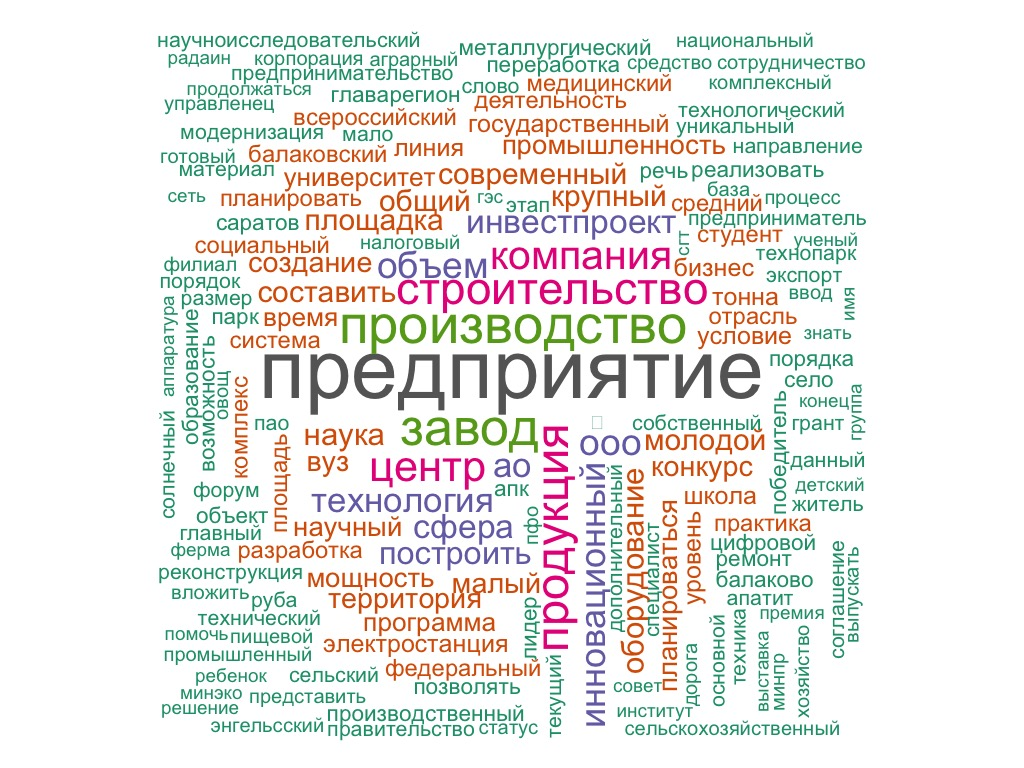
\includegraphics[width=0.8\linewidth]{Saratovskaya_Oblast_2021 Wordcloud.jpeg}

\caption{Облако слов для постов сообщества "Саратовская область" за 2021 год}

\label{fig:mpr}

\end{figure}





% Раздел "Заключение"
\conclusion



%Библиографический список, составленный вручную, без использования BibTeX
%
\begin{thebibliography}{99}
 \bibitem {1} Линник Л. А., Петросян М. М., Облако слов как метод компрессии информации научного текста // Наука. Информатизация. Технологии. Образование : материалы XIII международной научно-практической конференции, г. Екатеринбург, 24-28 февраля 2020 г. ---Екатеринбург : Издательство РГППУ, 2020. --- С. 99-108. 
\bibitem{2} Сапух Татьяна Викторовна Современные средства формирования лексических навыков учащихся на уроках английского языка (на примере облака слов) // АНИ: педагогика и психология. 2018. №3 (24).[Электронный ресурс]. URL: https://cyberleninka.ru/article/n/sovremennye-sredstva-formirovaniya-leksicheskih-navykov-uchaschihsya-na-urokah-angliyskogo-yazyka-na-primere-oblaka-slov (дата обращения: 03.09.2023).
\bibitem{3} Яркин П. А. Изучение экологического дискурса в контексте исследования экологического сознания // Экопсихологические исследования – 6: экология детства и психология устойчивого развития. 2020. №6.[Электронный ресурс]. URL: https://cyberleninka.ru/article/n/izuchenie-ekologicheskogo-diskursa-v-kontekste-issledovaniya-ekologicheskogo-soznaniya (дата обращения: 03.09.2023).
\bibitem{4} Journal of Teaching and Learning with Technology, Vol. 5, No. 1, July 2016, pp.16-32.
\bibitem{5} Davies, B.M., Mowforth, O.D., Khan, D.Z. et al. The development of lived experience-centered word clouds to support research uncertainty gathering in degenerative cervical myelopathy: results from an engagement process and protocol for their evaluation, via a nested randomized controlled trial. Trials 22, 415 (2021). [Электронный ресурс]. URL: https://doi.org/10.1186/s13063-021-05349-8 (дата обращения: 10.09.2023).
\bibitem{6} Umair, A., Masciari, E. Sentimental and spatial analysis of COVID-19 vaccines tweets. J Intell Inf Syst 60, 1–21 (2023). [Электронный ресурс]. URL: https://doi.org/10.1007/s10844-022-00699-4 (дата обращения: 25.09.2023).
\bibitem{7} Онлайн сервис формирования облака слов ``WordClouds.com''.  URL: https://www.wordclouds.com/ (дата обращения: 03.09.2023).
\bibitem{8} Онлайн сервис формирования облака слов ``wordcloud.online''. [Электронный ресурс]. URL: https://wordcloud.online/ (дата обращения: 04.09.2023).
\bibitem{9} Официальный сайт Python. [Электронный ресурс]. URL: https://www.python.org/
 \bibitem{10} Официальное сообщество VK ``Самарская область''. [Электронный ресурс]. URL: https://vk.com/samaroblast (дата обращения: 03.09.2023).
 \bibitem{11} Официальное сообщество VK ``Саратовская область''. [Электронный ресурс]. URL: https://vk.com/saratovoblgov (дата обращения: 03.09.2023).
 \bibitem{12} Официальное сообщество VK ``Республика Татарстан''. [Электронный ресурс]. URL: https://vk.com/nashtatarstan (дата обращения: 01.09.2023).
\bibitem{13} Список русских имён и фамилий. [Электронный ресурс]. URL: https://github.com/Raven-SL/ru-pnames-list/tree/master/lists (дата обращения: 20.09.2023).
\end{thebibliography}

%Библиографический список, составленный с помощью BibTeX
%
%\bibliographystyle{gost780uv}
%\bibliography{thesis}

% Окончание основного документа и начало приложений
% Каждая последующая секция документа будет являться приложением

\section{ПРИЛОЖЕНИЕ А}
\begin{verbatim}
\end{verbatim}
\end{document}
